\chapter{Оптико-электронные приборы}
\label{ch:tufte-design}

\newthought{Оптико-электронными приборами}\marginnote{\allcaps{ОПТИКО-ЭЛЕКТРОННЫЕ ПРИБОРЫ}} называются приборы, в которых информация об исследуемом или наблюдаемом объекте переносится оптическим излучением (содержится в оптическом сигнале), а ее первичная обработка сопровождается преобразованием этого излучения (оптического сигнала) в электрическую энергию (в электрический сигнал). 

В\marginnote{Далее может встречаться также термин <<оптические приборы>>, что будет подразумевать --- <<оптические приборы, содержащие в своем составе механические, электронные и оптические функциональные устройства и элементы>>, т.е. фактически --- ОЭП.} состав этих приборов входят как оптические, так и электронные звенья, причем и те и другие выполняют основные функции данного прибора, а не являются вспомогательными устройствами (например, узлами подсветки отсчетных шкал, устройствами термостабилизации).

ОЭП является сложной системой, включающей в себя большое число различных по своей физической природе и принципу действия звеньев -- аналоговых и цифровых преобразователей электрических сигналов, микропроцессоров, оптических, механических и электромагнитных узлов и др. Поэтому ОЭП часто называют оптико-электронными системами (ОЭС). 

Учитывая большое разнообразие ОЭП и их широкое применение в самых различных областях науки и техники  в курсе лекций рассмотрены общие для большинства ОЭП вопросы проектирования, достаточно общие и часто используемые на практике методы расчета и выбора основных параметров ОЭП, особенности конструкции и методы расчета параметров типовых узлов ОЭП.

Помимо исследуемого объекта (<<полезный>> излучатель) на рис.~\ref{pic:1OEPscheme} показаны и возможные на практике <<вредные>> излучатели (фоны, помехи). Взаимное расположение звеньев может быть и несколько иным. Отдельные звенья на практике представляют собой весьма сложные устройства, например, в состав источника излучения могут входить передающая оптическая система, фильтры, модулятор. Иногда в состав ОЭП не входят некоторые из перечисленных звеньев. Это определяется, как правило, методом работы прибора.

Все ОЭП предназначены для получения информации об объектах окружающей среды, переносимой оптическими сигналами. Хорошо известны ОЭП, используемые для локации, исследования природных ресурсов, измерения оптических свойств различных объектов. Многие ОЭП работают в составе следящих систем, используемых в навигации и ориентации, в системах технического зрения, устройствах автоматического контроля и управления, системах управления летательными аппаратами, системах наведения и во многих других устройствах для измерения линейных, угловых величин и определения координат объектов. Определенной спецификой обладают оптико-электронные системы противодействия и подавления оптических схем противника.

\begin{figure}[h!]
	\begin{center}
		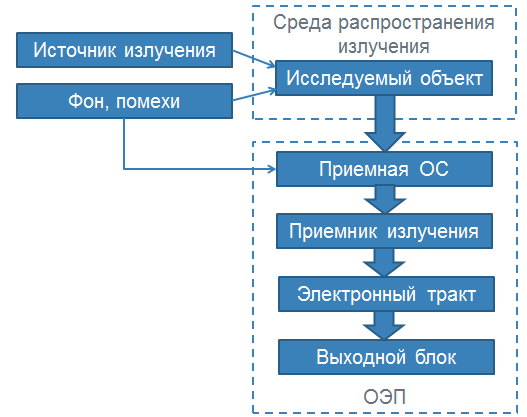
\includegraphics[width=0.8\linewidth]{OEPscheme.png}
		\caption{Обобщенная схема ОЭП}
		\label{pic:1OEPscheme}
	\end{center}
\end{figure}

Главный элемент --- оптическая система (ее сложно разработать, обеспечить нужное качество), которая определяется оптической схемой. С оптической схемы начинается разработка ОЭП.

\textsc{Оптической схемой}\marginnote{\allcaps{ОПТИЧЕСКАЯ СХЕМА}} называется графическое представление процесса изменения света в оптической системе.

Различия в принципах работы звеньев ОЭП, в способах обработки сигналов, проходящих через них, а также разнообразие условий эксплуатации ОЭП обусловливают сложность и многоступенчатость процесса проектирования этих приборов и требуют тщательного анализа как условий работы ОЭП, так и состояния имеющейся в распоряжении разработчика элементной базы.

\section{Классификация ОЭП}

Классификация ОЭП возможна по широкому кругу признаков в зависимости от принципов построения приборов и характера их применения (рис.~\ref{pic:1Classification}). К числу таких признаков могут быть отнесены параметры оптического сигнала, метод измерений, спектральный диапазон работы, режим работы, степень автоматизации, вид измерений, назначение и область применения, условия эксплуатации.

\begin{figure*}[h]
	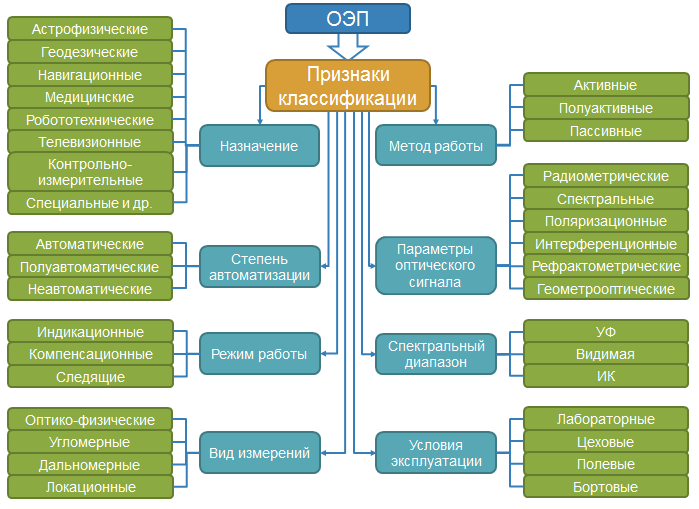
\includegraphics[width=\linewidth]{OEPclassification.png}
	\caption{Классификация ОЭП}
	\label{pic:1Classification}
\end{figure*}

Как известно, в ОЭП носителем полезной информации служит оптический сигнал в виде потока излучения, являющийся функцией координат $(x, y, z)$ измеряемого объекта, спектрального состава излучения ($\lambda$), времени ($t$), состояния и положения плоскости поляризации излучения ($A_\text{п}$), т.е. $\Phi(x, y, z, \lambda, t, A_\text{п})$. 

По методу работы ОЭП с учетом особенностей их построения и возможности управления параметрами излучения ОЭП делят на:
\begin{itemize}
	\item активные (наблюдаемый объект освещается (с помощью передающей оптической системы) лазером, при этом часть отраженного излучения поступает на вход ОЭП);
	\item полуактивные (один источник освещает все объекты);
	\item пассивные (используется собственное излучение исследуемого объекта; тепловое  (отраженное) от других источников излучения (солнца, луны); рассеянное излучение атмосферы и подстилающей поверхности).
\end{itemize}

В зависимости от спектрального состава используемого излучения ОЭП подразделяют на приборы, работающие в следующих областях спектра:
\begin{enumerate}
	\item ультрафиолетовая (УФ)~--- 200--380~нм ;
	\item видимая --- 400--700~нм;
	\item инфракрасная (ИК) --- 700 нм--1~мм.
\end{enumerate}

В свою очередь, УФ делится на: УФ-А (400--315 нм), УФ-Б (315--280 нм), УФ-С: (280--10 нм). Излучение с длиной волны менее 200 нм называют вакуумным ультрафиолетом, так как излучение не распространяется из-за полного поглощения в атмосфере.

ИК диапазон условно разделяют на: ИК-А или ближний ИК (700--1400 нм), ИК-Б или средний ИК (1400--3000 нм), ИК-С или дальний ИК (3 мкм--1 мм).

По степени автоматизации различают ОЭП:
\begin{enumerate}
	\item автоматические, работающие без участия оператора (обычно в следящем режиме);
	\item полуавтоматические, функционирование которых частично зависит от действий оператора;
	\item неавтоматические, выходная информация которых рассчитана на восприятие оператором.
\end{enumerate}

Существенные различия в принципах построения, функционирования и обслуживания имеют ОЭП, работающие в различных условиях эксплуатации:
\begin{enumerate}
	\item лабораторные;
	\item цеховые;
	\item полевые;
	\item бортовые.
\end{enumerate}

Наиболее емким из приведенных признаков классификации является назначение (область применения). Практически невозможно найти область техники, где бы в настоящее время не применялись ОЭП. Поэтому в схеме классификации указаны только некоторые области техники, в которых применение ОЭП является решающим фактором их дальнейшего развития: 
\begin{enumerate}
	\item навигация (гирометры);
	\item геодезия (теодолит);
	\item астрофизика (телескопы);
	\item робототехника (система машинного зрения);
	\item телевизионная техника (подсветка и формирование изображения);
	\item медицина (микроскопы);
	\item контрольно-измерительная техника (интерферометры);
	\item военная техника (оптические прицелы).
\end{enumerate}

ОЭП внутри каждой из рассмотренных классификационных групп могут подразделяться по конструктивным, функциональным и иным признакам. Кроме того, между всеми классификационными признаками существуют прямые и косвенные связи. Например, контрольно-измерительные приборы могут быть угломерными, автоматическими, цеховыми.

\section{Основные критерии оценки качества ОЭП}

\newthought{Качеством прибора}\marginnote{\allcaps{КАЧЕСТВО ПРИБОРА}} называется совокупность свойств прибора, обуславливающих его пригодность удовлетворять определенные потребности в соответствии с его назначением. Для объективной оценки качества прибора его свойства характеризуют количественно~--- показателями качества.

\noindent
\textsc{Показатели качества}\marginnote{\allcaps{ПОКАЗАТЕЛИ КАЧЕСТВА}}~--- это комплекс показателей, используемых для оценки свойств прибора, а также решений, принимаемых на различных этапах проектирования. 
Оценка качества ОЭП связана с рассмотрением широкого круга показателей, представленных на рис.~\ref{pic:1QualityOEP}.

\begin{figure*}[h]
	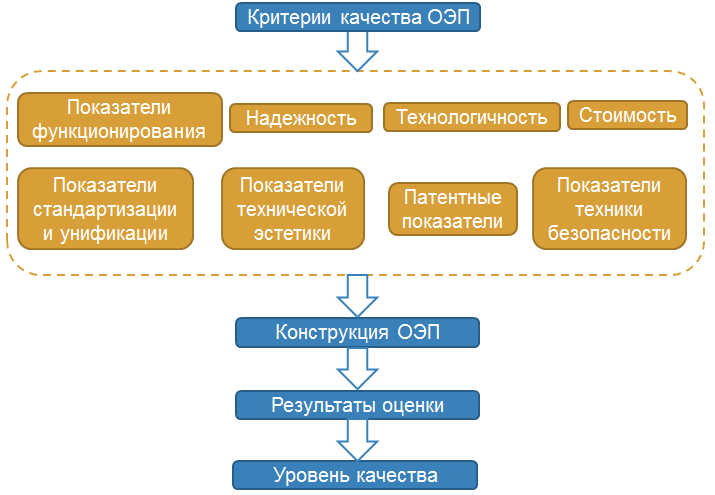
\includegraphics[width=0.7\textwidth]{1QualityOEP.png}
	\caption{Схема оценки качества ОЭП}
	\label{pic:1QualityOEP}
\end{figure*}

Всесторонняя оценка современных изделий может быть выполнена лишь при комплексном учете всех указанных показателей. Вместе с тем при проектировании разработчики чаще всего оценивают качество будущего прибора по показателям функционирования, надежности и технологичности.

\newthought{Показатели функционирования}\marginnote{\allcaps{ПОКАЗАТЕЛИ\break ФУНКЦИОНИРОВАНИЯ}} являются основными, они характеризуют техническую сущность прибора, и именно поэтому они стоят на первом месте в техническом задании.

Ввиду большого разнообразия ОЭП показатели функционирования могут быть самыми различными. Достаточно обобщенными являются информационные характеристики, к которым относят:
\begin{enumerate}
	\item входной язык, посредством которого осуществляется связь прибора с наблюдаемым или контролируемым объектом;
	\item энергия, необходимая для формирования единицы информации;
	\item функция преобразования, описывающая зависимость информативного параметра выходного сигнала от информативного параметра входного сигнала при номинальных значениях неинформативных параметров;
	\item выходной язык, посредством которого осуществляется связь прибора с потребителем информации;
	\item скорость выдачи информации прибором и восприятия ее потребителем (быстродействие).
\end{enumerate}

Наряду с перечисленными к показателям функционирования могут быть отнесены также вид потребляемой энергии и мощность потребления, габаритные размеры и масса прибора.

\newthought{Надёжность}\marginnote{\allcaps{НАДЁЖНОСТЬ}} определяется как свойство объекта сохранять во времени в установленных пределах значения всех параметров, характеризующих способность выполнить требуемые функции в заданных режимах и условиях применения, технического обслуживания, ремонта, хранения и транспортирования.

Сложность ОЭП, включающих оптические, механические и электронные узлы, требования к работоспособности этих приборов в резко изменяющихся условиях эксплуатации ставят перед конструктором задачу~--- создать прибор, обладающий высокой надежностью в течение всего срока службы.

Надёжность прибора зависит от количества и качества входящих в него элементов, условий работы (температуры, влажности, механических воздействий), схемного и конструктивного выполнения прибора, технологии изготовления и качества материала элементов.

\newthought{Технологичность}\marginnote{\allcaps{ПОКАЗАТЕЛИ\break ТЕХНОЛОГИЧНОСТИ}} деталей, узлов и конструкций, удобство сборки может быть охарактеризована следующими показателями: 
\begin{itemize}
	\item минимальными затратами труда на изготовление;
	\item минимальным ассортиментом средств изготовления;
	\item минимумом сложных и трудоемких производственных процессов;
	\item простотой подготовки производства;
	\item минимальным числом операций и временем их проведения;
	\item правильным выбором допусков на изготовление;
	\item простота монтажа деталей в узлы без дополнительной обработки;
	\item законченность узлов, входящих в прибор;
	\item простота сборки прибора в целом.
\end{itemize}

\textsc{Рациональный выбор материалов}: материалы, необходимые для изготовления деталей, следует выбирать с учетом не только функциональных и эксплуатационных особенностей прибора, но и технологии его изготовления. Для единичного производства целесообразно использовать материалы, хорошо поддающиеся обработке резанием. При крупносерийном и массовом производстве более экономичны способы изготовления без снятия стружки, что и определяет в значительной степени выбор материалов.

\textsc{Минимальная номенклатура элементов, материалов, полуфабрикатов} упрощает снабжение производства. 
Кроме того, необходимо иметь в виду, что некоторые детали и элементы часто не соответствуют специфике и профилю предприятия. В этих случаях целесообразнее идти по пути кооперации с другими предприятиями, чем осваивать производство соответствующих изделий.

\textsc{Обеспечение взаимозаменяемости деталей, узлов и блоков} предполагает идентичность конструктивных и присоединительных размеров, соединителей, а также входных и выходных параметров. Взаимозаменяемость позволяет обеспечить замену одного узла или блока другим без дополнительной подгонки и регулирования. Это обстоятельство имеет важное значение при сборке приборов, особенно при крупносерийном и массовом производстве, а также при обслуживании и ремонте приборов. Прежде всего необходимо стремиться к взаимозаменяемости электронных узлов и блоков. Взаимозаменяемость обеспечивается рациональными допусками на размеры и параметры узлов и блоков.

\textsc{Максимальная нормализация и унификация конструкций} основана на применении нормализованных, унифицированных или стандартизованных деталей и узлов. Нормализованные детали включены в нормаль данного предприятия или группы родственных предприятий. Унифицированные детали применяются на предприятиях всей отрасли промышленности. Стандартизованные детали используются на предприятиях различных отраслей промышленности.

Унифицированные и стандартизованные детали, узлы и блоки изготовляются централизованно, что позволяет автоматизировать процесс их производства, обеспечить высокую надежность и минимальную стоимость. Показатели унификации и стандартизации характеризуют степень использования и применения в данном приборе стандартизованных, унифицированных и заимствованных узлов и деталей. Чем больше таких элементов будет в проектируемом приборе, тем меньше затраты на их конструирование, технологическую подготовку производства, выше, как правило, надежность функционирования, проще организовать обслуживание и ремонт.

\textsc{Обеспечение возможности изготовления деталей при единичном и мелкосерийном производстве на универсальном оборудовании} имеет смысл при изготовлении уникальных и экспериментальных приборов, для выпуска которых в единичных образцах или малыми сериями нецелесообразно делать специальную технологическую оснастку. Повысить качество таких приборов и уменьшить технологические и трудовые затраты на их изготовление можно путем использования типовых узлов и деталей, о которых говорилось выше.

\textsc{Простота и удобство выполнения сборки, монтажа и юстировки} имеет особое значение для качественной настройки прибора, как в заводских условиях, так и в процессе дальнейшего использования. При этом снижаются трудовые затраты и требования к уровню подготовки производственного и обслуживающего персонала, а также требования к сложности юстировочного и стендового оборудования.

\newthought{Эстетические показатели}\marginnote{\allcaps{ЭСТЕТИЧЕСКИЕ\break ПОКАЗАТЕЛИ}} характеризуют внешний вид прибора, его соответствие современному стилю, гармоничность сочетания отдельных элементов прибора друг с другом, соответствие формы прибора его назначению, качество и совершенство отделки внешних элементов, поверхностей и упаковки, выразительность и качество надписей, знаков, технической документации (проспекта, каталога, инструкции, паспорта).

\newthought{Патентно-правовые показатели}\marginnote{\allcaps{ПАТЕНТНО-ПРАВОВЫЕ ПОКАЗАТЕЛИ}} характеризуют степень новизны заложенных в ОЭП технических решений а также вопросы патентно-правовой  защиты и определяются патентоспособностью и патентной чистотой. Патентоспособным является решение, которое может быть признано изобретением в одной или нескольких странах. Патентной чистотой обладают решения, не попадающие под действие (не нарушающие прав) других патентов.

\newthought{Показатели техники безопасности}\marginnote{\allcaps{ПОКАЗАТЕЛИ ТЕХНИКИ БЕЗОПАСНОСТИ}} характеризуют степень защищенности людей и животных от опасного воздействия ОЭП (защита от электрического удара, электромагнитных полей, теплового воздействия, радиации, оптических излучений, шума, токсичных и газовых выделений, вибраций), а также самих приборов от климатических, механических, биологических и других воздействий на них. Такими показателями, например, являются категория и класс исполнения и эксплуатации.

\newthought{Экономические показатели}\marginnote{\allcaps{ЭКОНОМИЧЕСКИЕ\break ПОКАЗАТЕЛИ}} выражаются прежде всего в стоимости прибора. К основным факторам, определяющим стоимость прибора, относятся область применения, условия эксплуатации, технологичность конструкции, требования по надежности, серийность выпуска, стоимость материалов и комплектующих изделий, простота и удобство обслуживания, юстировок и ремонта. 

Экономические показатели характеризуют уровень затрат на производство и эксплуатацию ОЭП. Среди них выделяют полную себестоимость и оптовую цену прибора. 

\newthought{Эргономические показатели}\marginnote{\allcaps{ЭРГОНОМИЧЕСКИЕ\break ПОКАЗАТЕЛИ}} характеризуют степень приспособленности прибора к взаимодействию с человеком с позиции удобства работы, гигиены, безопасности труда. 

Эргономические показатели разделены на гигиенические (уровень шума, амплитуда и частота вибраций, уровень радиации, температура, степень загазованности, токсичности), антропометрические (размеры и расположение экранов, индикаторов, рукояток, наглазников, налобников, форма сиденья), психофизиологические (диапазоны усилий на рукоятках, скорость выполнения движений, уровень освещенности, цвет и яркость световых сигналов, тембр и сила звуковых сигналов), психологические (объем и интенсивность потока информации, количество и частота выполняемых операций, количество и расположение контрольных, сигнальных, управляемых элементов).

\newthought{Экологические показатели}\marginnote{\allcaps{ЭКОЛОГИЧЕСКИЕ\break ПОКАЗАТЕЛИ}} характеризуют степень вредного влияния на окружающую среду и ее загрязнение при изготовлении, эксплуатации и утилизации приборов.

\newthought{Передаточные системы ОЭП}\marginnote{\allcaps{ПЕРЕДАТОЧНЫЕ\break СИСТЕМЫ ОЭП}} выделяются по виду преобразуемого сигнала: механическая, оптическая и электронная.
